\subsubsection{\stid{5.03} LLNL ATDM SW Ecosystem \& Delivery: DevRAMP}

\paragraph{Overview}
The {\bf DevRAMP} (Reproducibility, Analysis, Monitoring, and Productivity
for Developers) is creating tools and services that multiply the
productivity of HPC developers through automation. The project has two
major software efforts:

\begin{enumerate}
    \item {\bf Spack} is a package manager for
    HPC~\cite{melara+:cug17,gamblin+:sc17-spack-tutorial,gamblin+:sc16-spack-tutorial,gamblin+:sc15,gamblin+:llnl-spack-tutorial-17,gamblin+:ecp18-spack-tutorial,gamblin:pp18-spack,gamblin:hpckp17,gamblin:fosdem18-compilers,gamblin:fosdem18-binary,gamblin:ecp18-spack-sotu,gamblin:eb-user-meeting18,becker+:hust16}. It
    automates the process of downloading, building, and installing
    different versions of HPC software packages and their dependencies.
    With Spack, facilities can manage complex, multi-user software
    deployments on supercomputers, and developers can keep their own
    dependencies up to date in a single-user environment. Spack enables
    complex applications to be assembled from components, lowers barriers
    to software reuse, and allows complex HPC environments to be
    reproduced easily. It is the glue that holds the ECP software
    ecosystem together.

    \item {\bf Sonar} is a data cluster and a software stack for
    performance monitoring and analysis. Sonar allows developers and
    facility staff to understand how supercomputers and applications
    interact. The system continuously aggregates data from system-level
    monitoring services, application-level measurement tools, and
    facility power and temperature meters.  Any facility user can log in,
    examine performance data and other data collected about their HPC
    jobs, and share it with other users. Our focus is on security for the
    services running on Sonar (e.g., JupyterHub), and on developing an
    easy-to-use query tool, which we call ScrubJay.
\end{enumerate}


\paragraph{Key  Challenges}
{\it Spack} makes HPC application complexity manageable. HPC simulation
codes are notoriously complicated, and installing a code on a new
platform is not a simple task.  Codes are not self-contained; they rely
on tens or even hundreds of {\it dependencies} to implement their
functionality. While dependencies allow us to leverage the work of others
through code reuse, integrating hundreds of dependencies in the same
application is a monumental challenge.  Dependencies may require
different configurations and versions of their own dependency libraries,
and codes must be built and tested with different implementations of
interfaces MPI, BLAS, and LAPACK. The space of possible builds is
combinatorial in size, and it can only be effectively managed through
automation.

{\it Sonar} aims to find the root causes of performance variability of
jobs that run at Livermore Computing.  A single application execution may
have a different runtime depending on the system it runs on, the file
system it uses, or other jobs running at the same time.  A single
application execution may not accurately characterize performance.  The
causes of this variability may include file system performance, per-node
power consumption, application code performance, and even processor
performance from node to node. To analyze and understand performance
variability, we must collect data from the HPC center {\it and} from jobs
running at the facility, but we cannot show all application- and
facility-level data to all users. We need hardened security and
fine-grained permissions to ensure that data on Sonar is kept safe.


\paragraph{Solution Strategy}
{\it Spack} addresses HPC software complexity in three ways. First, it
provides a powerful build system and a domain-specific language for
writing package recipes.  This allows HPC builds to be templated and
easily mapped to HPC architectures. It provides dependency resolution
infrastructure, including virtual dependencies, a full parameter system,
and a dependency resolver we call a {\it concretizer}. Together, these
allow developers to specify customize builds for their own environments
based on {\it abstract} descriptions, while Spack handles the tedious
aspects of integrating with a new machine. Finally, Spack is an online
service where package recipes can be shared and the HPC community can
leverage each others' effort to reuse software. One of Spack's greatest
strengths is its very active online contributor community.

{\it Sonar} is a data cluster, a data model, a set of monitoring tools,
and an analysis front-end for manipulating this data. To deploy this in
the Livermore Computing (LC) center, our project has focused on securing
all components of this stack so that they can be hosted as services in a
multi-tenant environment. We have deployed the Cassandra database, the
Spark parallel processing engine, a custom tool of our own called
ScrubJay, among other components. We have added integration that allows
each tool to use LC's user ids and groups with access control lists. In
the case of Jupyter Notebooks and other services that launch jobs, we are
also hardening the process launch infrastructure so that notebooks launch
on behalf of users run {\it as} those users in the LC environment.

\paragraph{Recent Progress}
Figure~\ref{fig:sonar-spack} (left) shows the progress so far on Sonar
deployment.  The Cassandra database, as well as data collection from
compute clusters, filesystems, and facility temperature data is complete.
We have also recently completed a full-center deployment of JupyterHub
for accessing the data in the cluster. We were able to deploy JupyterHub
by adding SSL encryption to links between the hub and each notebook; this
required us to build a custom certificate authority into JupyterHub.  We
are currently preparing to upstreaming our solution to the mainline
JupyterHub repository.
\begin{figure}[htb]
    \centering
    \includegraphics[height=1.5in]{projects/2.3.5-Ecosystem/2.3.5.03-LLNL-ATDM-Ecosystem/sonar}~~~~~~~
    \includegraphics[height=1.5in]{projects/2.3.5-Ecosystem/2.3.5.03-LLNL-ATDM-Ecosystem/spack-fetch}
    \caption{
        \label{fig:sonar-spack} Sonar deployment (left) and
        Spack binary packaging (right).
    }
\end{figure}

We recently added the capability to create relocatable binary packages to
Spack~(Figure~\ref{fig:sonar-spack}, right).  Spack typically builds all
of its packages from source, as this is the de-facto software
distribution method for HPC systems. Recent additions to Spack allow us
to package even HPC software in optimized binary form, and to install in
minutes what could previously take hours. We are currently working on
making Spack's dependency resolution algorithm more robust to handle more
aggressive use of binary packages. Figure ~\ref{fig:concretize} shows the
current Spack concretizer, which will only reuse binaries that exactly
match a client-side concrete spec. The new version will allow Spack to
consider available remote binaries at install time, and to search more
aggressively through available binaries for usable dependencies. This
will mean even less rebuilding of software, and for HPC systems, this
means we will be able to match optimized binaries to the machine.

\begin{figure}[htb]
    \centering
    \includegraphics[width=\textwidth]{projects/2.3.5-Ecosystem/2.3.5.03-LLNL-ATDM-Ecosystem/spack-concretizer}
    \caption{\label{fig:concretize}
        Spack concretizer design changes.
    }
\end{figure}


\paragraph{Next Steps}
\begin{enumerate}

    \item {\bf Securing Kafka for Sonar.}  Sonar will ingest application
    data from the filesystem using a tool called Kafka. Kafka is a
    streaming communication infrastructure; it runs as a daemon and
    reliably transfers data from files to a database.  Kafka typically
    runs as a single user, but HPC centers are multi-tenant
    installations.  We will be adding functionality to ensure that Kafka
    preserves the identity of file owners in the filesystem when it
    ingests data into the database.

    \item {\bf Spack release testing and binary hosting.} Spack serves as
    a repository for package recipes, but we do not have any automated
    build testing of packages included in the Spack repository.  To
    increase the robustness and reliability of Spack, we are adding
    automation for building all packages in each Spack release, and for
    creating binary packages from such builds. We aim to provide binary
    packages for common configurations of Spack packages.
\end{enumerate}

\newpage 
\subsubsection{\stid{5.03} LLNL ATDM SW Ecosystem \& Delivery: Flux}

\paragraph{Overview}
{\bf Flux} is a next-generation workload management
framework for HPC~\cite{flux}. Flux maximizes scientific throughput
by assigning the scientific work requested by HPC users--–also
known as jobs or workloads--–to available resources that complete
the work, a method called scheduling. Using its highly scalable
breakthrough approaches of fully hierarchical scheduling and
graph-based resource modeling, Flux manages a massive number
of processors, memory, GPUs, and other computing system
resources--–a key requirement for exascale computing and beyond. 
A job is typically expressed in a script that contains
a formal specification for resource requests, identifies
applications (for instance, multi-physics simulation software
to run simultaneously across resources) along with their
input data and environment, and describes how to deliver
the output data. Modern scientific computing campaigns
contain numerous interconnected and dependent tasks with
disparate resource requirements. The composition of these
numerous interdependent tasks can be spread across many jobs,
as well as within each job, and is often referred to as a scientific
workflow (as distinct from a single job or workload). Assigning
resources to such modern workflows requires highly scalable
scheduling as well as performant communication and coordination
across hundreds of thousands of jobs, which could not be
accomplished with traditional HPC schedulers. Flux solves this
critical problem and has provided innovative solutions
for modern workflows for many scientific and engineering
disciplines.

\paragraph{Key  Challenges}
The workload manager is responsible for efficiently
delivering compute cycles of HPC systems to multiple users while considering their
diverse resource types---e.g., compute racks and nodes, central and graphics
processing units (CPUs and GPUs), multi-tiered disk storage
%
However, two broad technical trends are making even the best-in-class
products significantly ineffective.
%
The first trend is the evolution of workloads for HPC. With the convergence
of conventional HPC with new simulation, data analysis, machine learning (ML),
and artificial intelligence (AI) approaches, researchers are ushering in
new scientific discoveries. But this evolution also produces computing
workflows---often comprising many distinct tasks interacting with one
another---that are far more complex than traditional products
can sufficiently manage.
%
Second, hardware vendors have steadily introduced
new resource types and constraints into HPC systems.
Multi-tiered disk storage, CPUs and GPUs,
power efficiency advancements, and other hardware components have gained
traction in an era in which no single configuration reigns. Many HPC
architectures push the frontiers of compute power with hybrid (or
heterogeneous) combinations of processors.
The workload management software must manage and consider {\em extremely heterogeneous} computing
resources and their relationships for scheduling in order to realize a
system's full potential.
%

\paragraph{Solution Strategy}
Flux solves the key technical problems
that emerge from these trends.
It combines {\em fully hierarchical resource management}
with {\em graph-based scheduling} to improve
the performance, portability, flexibility,
and manageability of the scheduling
and execution of both standard and
complex scientific workflows on a wide range of HPC systems.
\begin{figure}[ht]
   \subfloat[Conventional Paradigm]{
        \begin{minipage}[c][1\width]{
           0.48\textwidth}
            \centering
            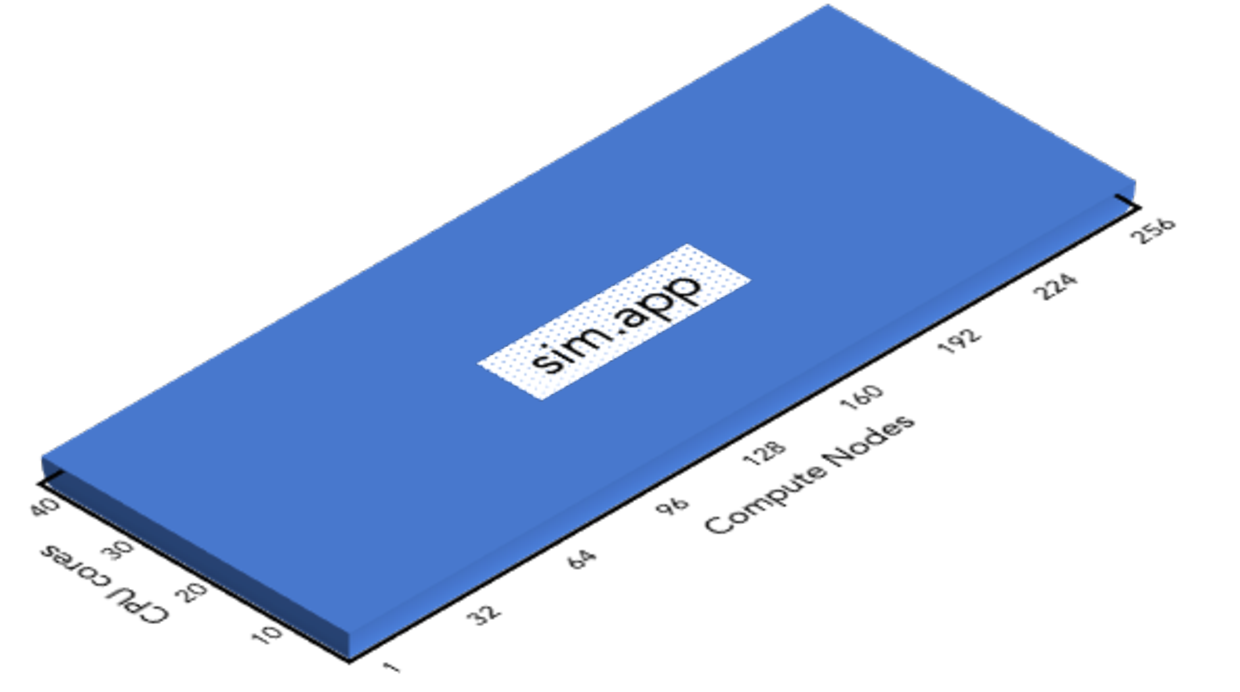
\includegraphics[width=1.1\textwidth]{projects/2.3.5-Ecosystem/2.3.5.03-LLNL-ATDM-Ecosystem/Old}
            \label{fig:old}
         \end{minipage}}
  \hfill
   \subfloat[Emerging Paradigm] {
         \begin{minipage}[c][1\width]{
            0.48\textwidth}
            \centering
            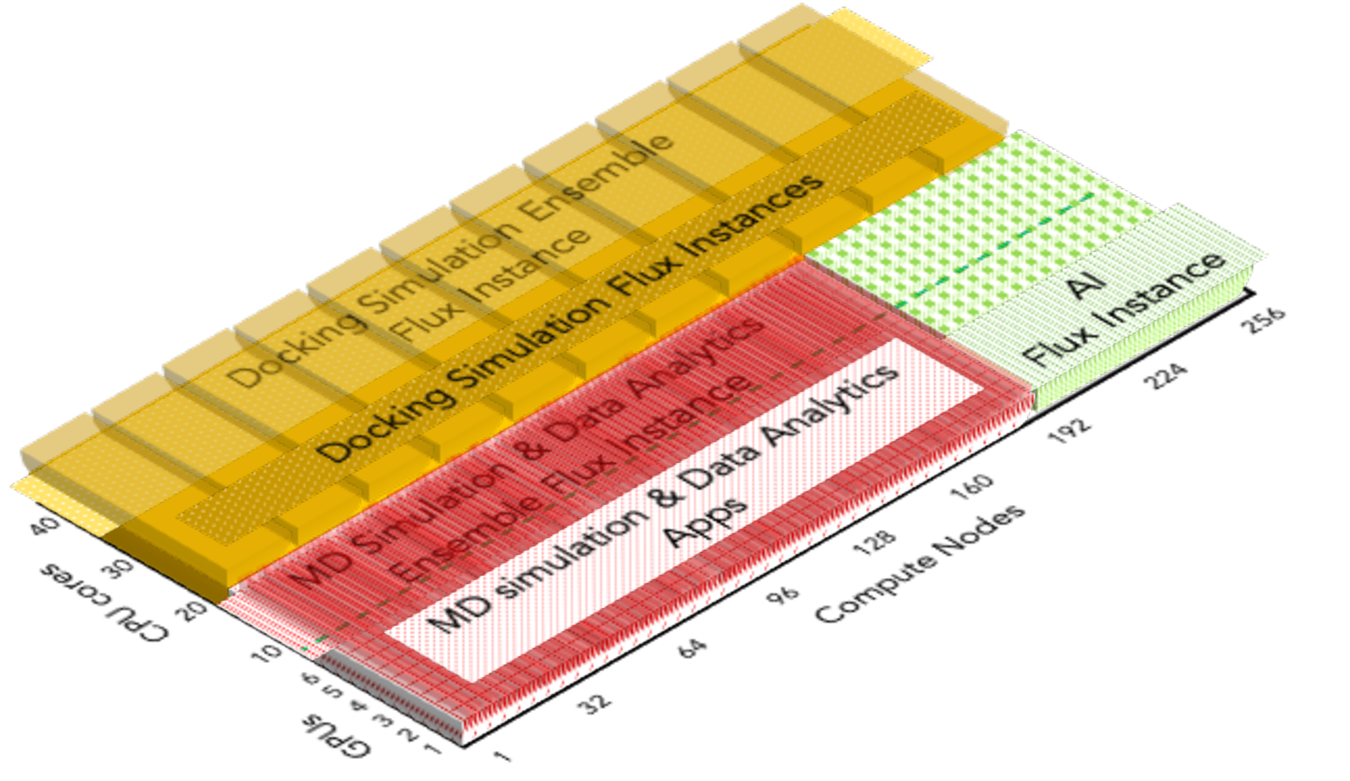
\includegraphics[width=1.1\textwidth]{projects/2.3.5-Ecosystem/2.3.5.03-LLNL-ATDM-Ecosystem/New}
            \label{fig:new}
         \end{minipage}}
 \caption{An illustration of how the computing resources allocated
to a job---as granted by the HPC workload manager---differs between
conventional and emerging scientific workflows. The notional X-axes
depict the compute node IDs allocated to the job and Y-axes depict
the IDs of computing resources in each of these nodes. (a) The conventional paradigm
requires only a single parallel simulation application to run; (b) The emerging paradigm often requires many different types of tasks such as an ensemble of molecular dynamic (MD) parallel simulation applications and another ensemble of docking simulation applications along with {\em in situ} data analysis for the MD ensemble while these tasks are driven by an AI.}
 \label{fig:layout}
 \end{figure}
Figure~\ref{fig:layout} visually contrasts
the complexity of the conventional and
new or emerging HPC paradigms in terms of
how they utilize the resources allocated
by the system's workload manager.
Nearly all existing products were designed
when the workflows were much simpler
as shown in Figure~\ref{fig:old}.
Yet, these solutions have significant difficulties with
the emerging paradigm exemplified
by Figure~\ref{fig:new},
as well as with connecting and coordinating jobs.
These problems have led users to develop their own {\em ad hoc}
custom scheduling and resource management software or use tools
that perform only workflow management or only scheduling.
However, accomplishing sufficient job coordination {\em without}
first-class support from a workload manager
like Flux has already proven to be difficult
for either approach.
Perhaps more importantly, developing and maintaining {\em ad hoc} management
software---especially in this era of ever-evolving HPC hardware
architectures---has quickly become prohibitively expensive for
supercomputing application teams.
With Flux, a job script with multiple
tasks submitted on a heterogeneous HPC system
remains simple, requiring only a few more lines within
the script.


\paragraph{Recent Progress}
Spurred by the growing convergence of conventional HPC and new simulation,
data analysis, and ML/AI techniques, the computational science community
has been embracing much more diverse workflow solutions than ever before.
Flux has been able to provide innovative solutions for researchers,
and our development team has brought a co-design strategy to early
scientific use cases to improve functionality, performance, and scalability.

\paragraph{Next Steps}
Development of the system instance of Flux, which will enable it to
be the primary system workload manager on exascale-computing-class supercomputers
by 2023, is actively being pursued as additional features
and performance/scalability tuning, commensurate with the capabilities
of then these systems, are required.
\begin{enumerate}
    \item Add support for HPE's Rabbit-based multi-tiered storage scheduling and management within Flux;

    \item Add support for Common Tools Interface (CTI)-based tool launching to enable HPE's proprietary code-development tools;

    \item Variorum-enabled power monitoring/capping subsystem;

    \item Respond agilely to the emerging needs of existing and new workflow customers. 

\end{enumerate}

